% Cap�tulo 4
\chapter{Modelo de sentimento - Estudo de caso com os pré-candidatos à Presidência do Brasil de 2018}

\section{Descrição do estudo de caso}

Após definido o modelo de análise de sentimento a ser utilizado neste trabalho, sua aplicação se dá em um estudo de caso, realizado nas redes sociais, sobre o sentimento dos comentários a respeito dos prováveis candidatos à Presidência do Brasil de 2018. 

Este estudo conta com coleta de dados nessas redes, filtrados de acordo com os nomes desses pré-candidatos e, após isso, é feita a análise de sentimento do texto coletado.

Tal feito, ocorre em duas etapas. Uma primeira, na qual a quantidade de dados coletados são padronizados para todos os pré-candidatos e, na segunda, essa quantidade é aleatória para cada um, pois o objetivo é saber o volume que cada um apresenta, durante o período de uma hora, com coleta em \textit{streaming}.

\subsection{Objetivos do estudo de caso}

O objetivo deste estudo é analisar se nas redes sociais, os comentários a respeito dos possíveis candidatos às eleições à Presidência, do Brasil, no ano de 2018, são positivos, negativos ou apresentam um valor semântico neutro, ou seja, não opinativo.

\subsection{Seleção dos participantes do caso estudado}

De acordo com o cronograma do Tribunal Superior Eleitoral (TSE), para as eleições de 2018 no Brasil, o registro oficial dos candidatos estará definido no mês de agosto desse ano. 

Embora, não seja possível conhecê-los no momento da execução do estudo de caso aqui proposto, a escolha dos nomes, os quais as coletas e análises são feitas, tem como embasamento matérias produzidas por alguns dos principais portais de notícias brasileiros que, relatam quem são os principais pré-candidatos à Presidente da República brasileira. 

Os nomes escolhidos, são: Luiz Inácio Lula da Silva do PT (Partido dos Trabalhadores), Jair Bolsonaro do PSL (Partido Social Liberal), Geraldo Alckmin do PSDB (Partido da Social Democracia Brasileira), Ciro Gomes PDT (Partido Democrático Trabalhista) e Marina Silva do partido Rede Sustentabilidade, tirados de matérias nos portais: G1, Folha, Estadão, R7, UOL, BBC Brasil.

\section{Execução do estudo de caso com quantidade de dados padronizada}

\subsection{Procedimento de coleta de dados}

Os dados coletados advêm da rede social Twitter. Para possibilitar a busca desses dados é necessário executar as etapas de, criação de um aplicativo, autenticação para permissão de acesso via cliente HTTP e busca de dados de acordo com parâmetros passados nas requisições às API’s.


No Twitter é necessário cadastrar-se no endereço https://apps.twitter.com. Após isso, é possível criar um novo aplicativo e ter acesso aos parâmetros que são necessários nas requisições à API, como é possível ver na figura \ref{fig:criacaoAppTwitter}. 

\begin{figure}[h]
    \centering
    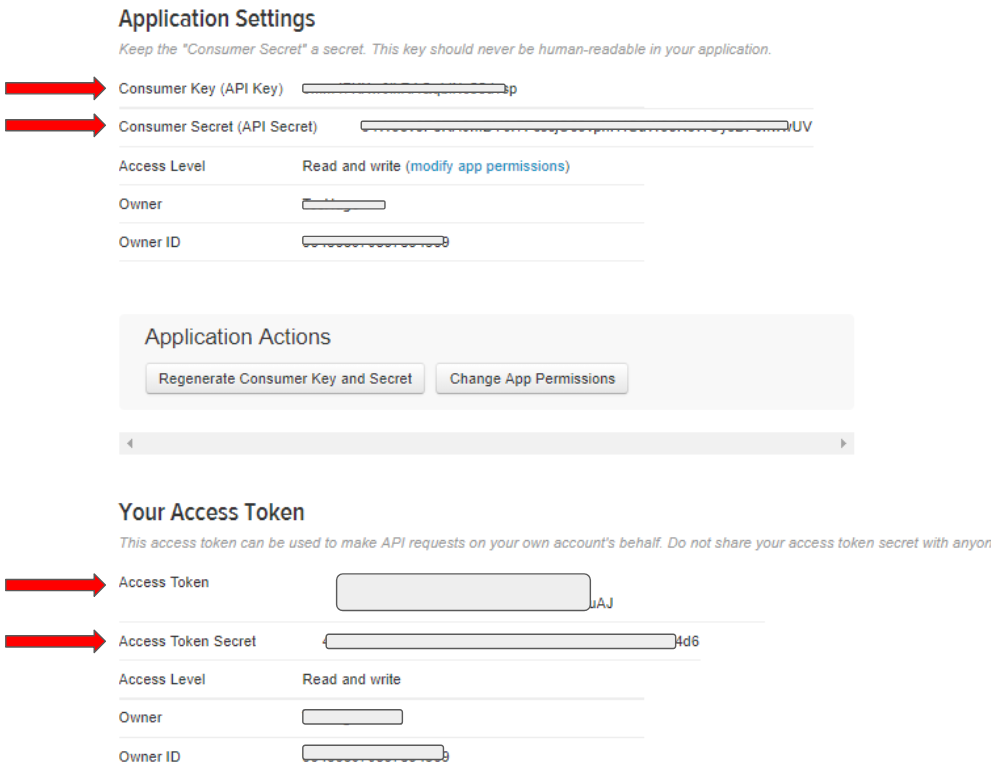
\includegraphics[\textwidth,height=10cm]{imagens/criacaoAppTwitter.png}
    \caption {Parâmetros para autenticação com a API do Twitter.}
    \source{Fonte: Criado pelo autor (2018)}
    \label{fig:criacaoAppTwitter}
\end{figure}

\begin{table}[!htb]
   \textsf{\caption{Parâmetros de coleta no Twitter.}}
   \centering
   \medskip

    \begin{tabular}{ |p{4cm}|p{3cm}|p{3cm}|p{3cm}|  }
     \hline
     \multicolumn{4}{|c|}{Parâmetros de coleta no Twitter} \\
     \hline
       \diagbox{Candidato}{Parâmetro} & Período de coleta & Quantidade de Tweets coletados & Termos da pesquisa\\
     \hline
     
     \hline
      Lula (PT)   & 30 a 31 de Maio de 2018 & 100 &  luiz inacio lula da silva \\
     \hline
     
      \hline
      Bolsonaro (PSL)   & 30 a 31 de Maio de 2018 & 100 & jair bolsonaro  \\
     \hline
     
      \hline
      Alckmin (PSDB)   & 30 a 31 de Maio de 2018 & 100 & geraldo alckmin  \\
     \hline
     
      \hline
      Ciro (PDT)   & 30 a 31 de Maio de 2018 & 100 & ciro gomes  \\
     \hline
     
      \hline
      Marina (REDE)   & 30 a 31 de Maio de 2018 & 100 &  marina silva \\
     \hline

    \end{tabular}
    \label{table:2}
\end{table}

Em seguida a conexão com a API é realizada via código Python utilizando a biblioteca \textit{python-twitter}, passando como parâmetros o \textit{Consumer Key}, \textit{Consumer Secret}, \textit{Access Token}, \textit{Access Token Secret}, para obter permissão de acesso como cliente HTTP.


Com isso, uma requisição é feita, passando os parâmetros de filtragem das informações que, devem ser coletadas. Esses parâmetros são os nomes dos pré-candidatos, datas de início e fim de quando as mensagens foram postadas na rede social, criando um intervalo temporal, geolocalização delimitando a área de onde os usuários postaram na rede e idioma no qual a mensagem está.

Os parâmetros de coleta foram padronizados de acordo com a tabela da seção \ref{table:2}. Todos os dados, dos cinco pré-candidatos, foram coletados de acordo com seus respectivos nomes, durante o período de um dia (30 a 31 de Maio de 2018) e com o número máximo de cem tweets (devido limitação que a API do Twitter impõe para a coleta de busca por termo).

Esse procedimento é realizado com o seguinte trecho de código do sistema:

Leitura das credenciais, necessárias para autenticação com o Twitter, do arquivo env.ini. Esse arquivo é responsável por manter os valores necessários que são utilizados pelo sistema (uma espécie de arquivo com variáveis de ambiente).
\begin{code}
\begin{minted}
[
frame=lines, linenos,fontsize=\footnotesize
]
{python}

from env.env import lerEnv

Config = lerEnv()

CONSUMER_KEY = Config.get("credenciaisTwitter", "CONSUMER_KEY")
CONSUMER_SECRET = Config.get("credenciaisTwitter", "CONSUMER_SECRET")
OAUTH_TOKEN = Config.get("credenciaisTwitter", "OAUTH_TOKEN")
OAUTH_TOKEN_SECRET = Config.get("credenciaisTwitter", "OAUTH_TOKEN_SECRET")
\end{minted}
\label{code:credenciaisTwitter}
\end{code}


Importação das funções responsáveis à autenticação.
\begin{minted}
[
frame=lines, linenos
]
{python}

from autenticacao.autenticacaoTwitter import oauth_login
from analiseSentimental.coletarTwitter import coletar_por_termos

\end{minted}

Autenticação na API do Twitter.
\begin{minted}
[
frame=lines, linenos,fontsize=\footnotesize
]
{python}

twitter_oauth = oauth_login(CONSUMER_KEY, 
                            CONSUMER_SECRET, 
                            OAUTH_TOKEN, 
                            OAUTH_TOKEN_SECRET)

\end{minted}

Realização de colerta de dados, utilizando a biblioteca python-twitter, recebendo os dados de resposta no formato JSON.
\begin{minted}
[
frame=lines, linenos
]
{python}

candidato = coletar_por_termos(twitter_oauth, ['nome candidato']) 

\end{minted}


\subsection{Procedimento de análise de dados}



    \subsubsection{Seleção dos dados de interesse}

	Embora as informações, advindas, do Twitter se mantenham,praticamente imutáveis, durante todo o procedimento de análise que o sistema realiza, a estrutura de dados é mudada. Ao requisitar os dados à API, as informações são mantidas em um objeto do tipo \textit{dict} então, para facilitar a realização da análise de sentimento, esta estrutura é convertida em um objeto do tipo, \textit{DataFrame}. 
	
	Em seguida os dasos a serem tratados, são pasados a função responsável por tal feito. Como demostra-se no código a seguir.

\begin{minted}
[
frame=lines, linenos
]
{python}

import pandas
dfCandidato = pandas.DataFrame(candidato['statuses'])
from analiseSentimental.analiseSentimental import limpar_texto_dataset
corpus = limpar_texto_dataset(dfCandidato, 'text', len(dfCandidato))

\end{minted}

                
    \subsubsection{Tratamento dos dados selecionados}

          Após convertida a estrutura de dados, todas as linhas do campo \textit{text} são tratadas, para a análise posterior. Este processo consiste de sete etapas que, são explicadas junto ao código a seguir.

A função limpar\_texto\_dataset, recebe como parâmetro o dataset da coleta realizada no Twitter, o nome da coluna, na qual, os dados serão tratados e a quantidade de dados a serem prontos para análise.
\begin{minted}
[
frame=lines, linenos
]
{python}

def limpar_texto_dataset(dataset, coluna, qtdLinhas):

\end{minted}

É criada uma lista que receberá os textos depois de limpos.
\begin{minted}
[
frame=lines, linenos
]
{python}

corpus = []

\end{minted}

Para cada texto contido na lista a ser tratada...
\begin{minted}
[
frame=lines, linenos
]
{python}

for i in range(0, qtdLinhas):

\end{minted}

É removido qualquer palavra que não contenha os caracteres de A até maiúsculos e acentuadas, de a até z minúsculos e acentuadas.
\begin{minted}
[
frame=lines, linenos
]
{python}

linha = re.sub('[^A-Za-zá-ú]', ' ', dataset[coluna][i])

\end{minted}

Todo texto é codificado no formato UTF-8.
\begin{minted}
[
frame=lines, linenos
]
{python}

linha = dataset[coluna][i].encode('utf-8')

\end{minted}

Logo após, os caracteres de suas palavras são transformadas em minúsculos.
\begin{minted}
[
frame=lines, linenos
]
{python}

 linha = linha.lower()

\end{minted}

As palavras são separadas por espaço em branco.
\begin{minted}
[
frame=lines, linenos
]
{python}

linha = linha.split()

\end{minted}

São retiradas as \textit{stopwords} do texto (palavras que não possuem influência subjetiva na frase).
\begin{minted}
[
frame=lines, linenos
]
{python}

linha = [palavra for palavra in linha
            if not palavra in stopwords.words('portuguese')]


\end{minted}

Por fim essa nova frase, já tratada, é acrescentada ao dataset. Para que assim, outro \textit{tweet} possa ser tratado.
\begin{minted}
[
frame=lines, linenos
]
{python}

linha = str(' '.join(linha))
corpus.append(linha)
    
return corpus
\end{minted}


        \subsubsection{Dicionário de sentimentos}
        
O dicionário, utilizado para análise de sentimento, é fruto do trabalho de \cite{dicionarioSentimento}. Nele estão contidas 47424 palavras classificadas com valores entre -1, 0 ou 1 que, representam seu valor sentimental. O valor -1, representa uma palavra negativa, 0 um palavra neutra e 1, positiva. Uma pequena parte do dicionário é mostrada na figura \ref{fig:dicionarioSentimento}.

\begin{figure}[h]
    \centering
    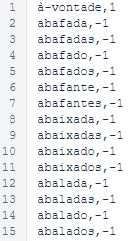
\includegraphics[\textwidth,height=5cm]{imagens/dicionario.png}
    \caption {Dicionário de palavras com valor de sentimento.}
    \source{Fonte: Criado pelo autor (2018)}
    \label{fig:dicionarioSentimento}
\end{figure}


   \subsubsection{Análise de sentimentos}
        
	A análise de sentimentos realizada, neste trabalho, se baseia em uma abordagem supervisionada. Em síntese, os dados textuais (um \textit{tweet} por vez), após tratamento, são imputados em uma ferramenta responsável por avaliar e devolver um valor inteiro, correspondente ao sentimento daquele texto. Se positivo, esse valor é maior que zero, se neutro é zero e se negativa, possui valor menor que zero.

Abaixo, o código em Python é explicado.

São importadas as funções necessárias à análise. O dicionário com as palavras de sentimento é preparado e uma coluna que, contém os valores de sentimento de cada \textit{tweet}, é criada.
\begin{minted}
[
frame=lines, linenos,fontsize=\footnotesize
]
{python}

from analiseSentimental.analiseSentimental import calcularSentimento, frase_em_token

dicionario = pandas.read_csv("arquivosTeste/sentilex-reduzido.txt", header=None)
dfCandidato['sentimento'] = ''

\end{minted}

Depois, cada mensagem do Twitter, é dividida em palavras. E o valor do sentimento é calculado e pôsto no \textit{tweet} correspondente. O cálculo desse valor é explicitado no próximo trecho de código.
\begin{minted}
[
frame=lines, linenos
]
{python}

for i in range(0, len(corpus)):

    texto = frase_em_token(corpus[i])
    dfCandidato['sentimento'][i] = calcularSentimento(texto, dicionario)

\end{minted}

Por fim, a função, calcularSentimento, recebe o texto a ser valorado e o dicionário de palavras.
\begin{minted}
[
frame=lines, linenos
]
{python}

def calcularSentimento(texto, dicionario):
\end{minted}

É declarado um contador, responsável por guardar o valor de sentimento durante as iterações que ocorrerão.
\begin{minted}
[
frame=lines, linenos
]
{python}

  valorSentimento = 0
\end{minted}

Assim, cada palavra do \textit{tweet} é comparada com cada palavra do dicionário. Se elas forem iguais, uma outra estrutura de dados (matchComDicionario) recebe os registros do dicionário. No final, todos os valores de sentimento das palavras que são iguais entre o dicionário e o texto, são somados ao valor da variável que serve como contador. E o valor de sentimento do texto é retornado.
 
\begin{minted}
[
frame=lines, linenos, fontsize=\footnotesize
]
{python}
 matchComDicionario = pandas.DataFrame()
                
for i in range(0, len(texto)):
    matchComDicionario=matchComDicionario.append(dicionario[dicionario[0]==texto[i]])
    
for j in range(0, len(matchComDicionario)):
   valorSentimento = valorSentimento + dicionario[1][j]

return valorSentimento

\end{minted}

\section{Execução do estudo de caso com \textit{streaming} de dados}

\subsection{Procedimento de coleta de dados}

Assim como na coleta realizada com quantidade padrão de \textit{tweets}, é necessário que se crie um aplicativo como desenvolvedor. Como é explicado na seção 4.2.1 e mostrado na figura \ref{fig:criacaoAppTwitter}.

Depois de criar o aplicativo, a coleta de dados, via \textit{streaming}, é efetuada com o seguinte trecho de código.

\begin{minted}
[
frame=lines, linenos, fontsize=\footnotesize
]
{python}
from tweepy.streaming import StreamListener
from tweepy import OAuthHandler
from tweepy import Stream

class Listener(StreamListener):

    def on_data(self, data):
        print data
        arquivo = open('./resultados/twitter/streamingTwitter.json', 'a')
        arquivo.write(data) 
        arquivo.write('\n')
        arquivo.close()

        return True

    def on_error(self, status):
        arquivo = open('./resultados/twitter/streamingTwitterErro.json', 'a')
        arquivo.write(status) 
        arquivo.write('\n')
        arquivo.close()
        print status


if __name__ == '__main__':
    
    termos = ['luiz inacio lula da silva', 
              'jair bolsonaro', 
              'marina silva', 
              'ciro gomes', 
              'geraldo alckmin']

    listener = Listener()
    auth = OAuthHandler(CONSUMER_KEY, CONSUMER_SECRET)
    auth.set_access_token(OAUTH_TOKEN, OAUTH_TOKEN_SECRET)
    stream = Stream(auth, listener)
    # locations = coordenadas da amplitude territorial de coleta
    # neste caso: Brasil.
    # São passados dois parâmetros: longitude e latitude (nessa ordem) do sul ao norte 
    stream.filter(track=termos, locations=[-52.875989,-31.754882,-51.469739,2.604407])
\end{minted}

Primeiramente, são importadas as bibliotecas necessárias.
\begin{minted}
[
frame=lines, fontsize=\footnotesize
]
{python}
from tweepy.streaming import StreamListener
from tweepy import OAuthHandler
from tweepy import Stream
\end{minted}

A classe \textit{Listener} é criada e recebe a injeção de dependência da classe  \textit{StreamListener}, que possui dois métodos: \textit{on\_data} e  \textit{on\_error}.

O primeiro “escuta” a API do Twitter e escreve as respostas, vindas no formato JSON, em um arquivo dentro do diretório do projeto. O segundo, é responsável por lidar com os erros que podem ocorrer durante a coleta. E também são escritos em um arquivo dentro do projeto do sistema.
\begin{minted}
[
frame=lines, fontsize=\footnotesize
]
{python}
class Listener(StreamListener):

    def on_data(self, data):
        print data
        arquivo = open('./resultados/twitter/streamingTwitter.json', 'a')
        arquivo.write(data) 
        arquivo.write('\n')
        arquivo.close()

        return True

    def on_error(self, status):
        arquivo = open('./resultados/twitter/streamingTwitterErro.json', 'a')
        arquivo.write(status) 
        arquivo.write('\n')
        arquivo.close()
        print status

\end{minted}

No método de inicialização, são definidos os termos da coleta. Neste caso os cinco nomes dos pré-candidatos.
\begin{minted}
[
frame=lines, fontsize=\footnotesize
]
{python}

if __name__ == '__main__':
    
termos = ['luiz inacio lula da silva', 
          'jair bolsonaro', 
          'marina silva', 
          'ciro gomes', 
          'geraldo alckmin']


\end{minted}

Um objeto \textit{Listener} é criado, a autenticação com a API de \textit{streaming} é efetivada, ao passar os quatro parâmetros necessários, que são obtidos, utilizando o código da seção \ref{code:credenciaisTwitter}. Então, um objeto que, realizará a coleta de dados em fluxo, é instanciado passando o \textit{Listener} e a autenticação.
\begin{minted}
[
frame=lines, fontsize=\footnotesize
]
{python}
    listener = Listener()
    auth = OAuthHandler(CONSUMER_KEY, CONSUMER_SECRET)
    auth.set_access_token(OAUTH_TOKEN, OAUTH_TOKEN_SECRET)
    stream = Stream(auth, listener)

\end{minted}

Por fim, é aberto um canal com a API de \textit{streaming} do Twitter, no qual os nomes dos pré-candidatos e a abrangência territorial, na qual os dados são buscados.

O parâmetro \textit{locations}, define essa abrangência. Sendo os dois primeiros valores a longitude e latitude de um determinado ponto ao sul e os dois seguintes a longitude e latitude de um ponto ao norte. Neste caso, são coordenadas do extremo sul do Brasil ao extremo norte.
\begin{minted}
[
frame=lines, fontsize=\footnotesize
]
{python}
stream.filter(track=termos, locations=[-52.875989,-31.754882,-51.469739,2.604407])
\end{minted}

\subsection{Procedimento de análise de dados}

Os dados de coleta, se vistos em um terminal de linha de comando, apresentam esta característica da figura \ref{fig:telaStreaming.png}.

\begin{figure}[h]
    \centering
    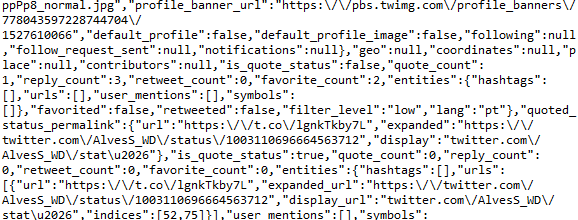
\includegraphics[width=0.95\textwidth]{imagens/telaStreaming.png}
    \caption {Tela de um terminal de linha de comando com dados de \textit{streaming} do Twitter.}
    \source{Fonte: Criado pelo autor (2018)}
    \label{fig:telaStreaming.png}
\end{figure}

Para possibilitar a legibilidade e análise desses dados, as seguintes etapas de tratamento, são executadas.

\begin{minted}
[
frame=lines, linenos, fontsize=\footnotesize
]
{python}
import pandas
from analiseSentimental.analiseSentimental import calcularSentimento, 
limpar_texto_streaming, 
definir_sentimento_dataset
                                                  
data=pandas.read_json(open('./resultados/twitter/streamingTwitter.json'), lines=True)

datasetLimpo = limpar_texto_streaming(data, 'text')

dicionario = pandas.read_csv("arquivosTeste/sentilex-reduzido.txt", header=None)
resultado = definir_sentimento_dataset(datasetLimpo, dicionario)

lula = resultado[resultado['text'].str.contains("luiz|inacio|lula")]
bolsonaro = resultado[resultado['text'].str.contains("jair|bolsonaro")]
marina = resultado[resultado['text'].str.contains("marina|silva")]
ciro = resultado[resultado['text'].str.contains("ciro|gomes")]
geraldo = resultado[resultado['text'].str.contains("geraldo|alckmin")]

from analiseSentimental.analiseSentimental import quantidade_sentimento
quantidade_sentimento(datasetPreCandidato) 

\end{minted}

A princípio, os métodos responsáveis por executar o código, são importados.
\begin{minted}
[
frame=lines, fontsize=\footnotesize
]
{python}
import pandas
from analiseSentimental.analiseSentimental import calcularSentimento, 
limpar_texto_streaming, 
definir_sentimento_dataset
                                                  
\end{minted}

Depois, os dados são lidos e armazenados em num \textit{DataFrame}.
\begin{minted}
[
frame=lines, fontsize=\footnotesize
]
{python}
data = pandas.read_json(open('./resultados/twitter/streamingTwitter.json'), lines=True)                                                  
\end{minted}

Com isso, os dados textuais que, serão analisados, são “limpos”. Retira-se pontuação, palavras sem valor subjetivo, muda-se o formato de codificação dos caracteres e transforma-os em minúsculos.
\begin{minted}
[
frame=lines, fontsize=\footnotesize
]
{python}
datasetLimpo = limpar_texto_streaming(data, 'text') 

# função responsável por isso
def limpar_texto_streaming(dataset, coluna):
                 
    for i in range(0, len(dataset)):
        texto = re.sub('[^A-Za-zá-ú]', ' ', dataset[coluna][i])
        texto = dataset[coluna][i].encode('utf-8')
        texto = texto.lower()
        
        texto = texto.split()

        texto = [palavra for palavra in texto
                         if not palavra in stopwords.words('portuguese')]
        
        texto = frase_em_token(texto)
        
        dataset[coluna][i] = " ".join(texto)   
    
    return dataset
                                           
\end{minted}

Então, lê-se o dicionário de palavras com valor de sentimento.
\begin{minted}
[
frame=lines, fontsize=\footnotesize
]
{python}
dicionario = pandas.read_csv("arquivosTeste/sentilex-reduzido.txt", header=None)                                               
\end{minted}

Assim, é acrescida uma coluna no dataserLimpo, que receberá o valor de sentimento de cada texto.
\begin{minted}
[
frame=lines, fontsize=\scriptsize
]
{python}
resultado = definir_sentimento_dataset(datasetLimpo, dicionario)    

# função responsável por isso
def calcularSentimento(texto, dicionario):
    
    texto = texto.split()
    valorSentimento = 0
    matchComDicionario = pandas.DataFrame()
                
    for i in range(0, len(texto)):
        matchComDicionario = matchComDicionario.append(dicionario[dicionario[0] == texto[i]])
        
    for j in range(0, len(matchComDicionario)):
       valorSentimento = valorSentimento + dicionario[1][j]
    
    return valorSentimento
                                          
\end{minted}

Em seguida, um dataset para cada pré-candidato, é criado. Dividindo a quantidade total de informações coletadas, nos seus respectivos representantes.

\begin{minted}
[
frame=lines, fontsize=\footnotesize
]
{python}
lula = resultado[resultado['text'].str.contains("luiz|inacio|lula")]
bolsonaro = resultado[resultado['text'].str.contains("jair|bolsonaro")]
marina = resultado[resultado['text'].str.contains("marina|silva")]
ciro = resultado[resultado['text'].str.contains("ciro|gomes")]
geraldo = resultado[resultado['text'].str.contains("geraldo|alckmin")]                                            
\end{minted}

Finalmente, são calculadas as quantidades de sentimentos, dentre positivos, negativos e neutro, para cada candidato.
\begin{minted}
[
frame=lines, fontsize=\footnotesize
]
{python}
from analiseSentimental.analiseSentimental import quantidade_sentimento
quantidade_sentimento(datasetPreCandidato)                                           
\end{minted}

Gerando uma resposta neste formato.
\begin{minted}
[
frame=lines, fontsize=\footnotesize
]
{python}
Out[1]: ['positivo - 6', 'neutro - 27', 'negativo - 1']                                         
\end{minted}

Após a coleta, tratamento e análise de sentimento dos dados, um mapa, contendo os locais, de onde os usuários postam no Twitter, é criado. Com o auxílio da biblioteca folium da linguagem Python, os dados de geolocalização são lidos e uma página em HTML, com o mapa e seus marcadores, é gerada automaticamente. Esse processo é executado com o seguinte código.

\begin{minted}
[
frame=lines, linenos, fontsize=\footnotesize
]
{python}
import folium
import pandas
import ast

dfCandidato=pandas.read_csv("resultados/twitter/resultadoComSentimento.csv",
index_col=0, encoding='utf-8')

map=folium.Map(location=[-15.681307, -47.939025],zoom_start=4,tiles='Mapbox bright')

for i in range(0, len(dfCandidato)):
    
    if str(dfCandidato['coordinates'][i]) != 'nan':
        
        dfCandidato['coordinates'][i] = ast.literal_eval(dfCandidato['coordinates'][i])
        
        corPonto = ''
        
        if dfCandidato['sentimento'][i] > 0:
            corPonto = 'green'
        elif dfCandidato['sentimento'][i] < 0:
            corPonto = 'red'
        else:
            corPonto = 'blue'
            
        popup = folium.Popup(dfCandidato['text'][i], parse_html=True)
            
        folium.Marker(
            # primeiro longitude depois latitude
            location=[ dfCandidato['coordinates'][i]['coordinates'][1], 
                       dfCandidato['coordinates'][i]['coordinates'][0]
                     ],
            icon=folium.Icon(color=corPonto),
            popup=popup,
        ).add_to(map)

map.save(outfile='templates/mapa.html') 

\end{minted}

De início, as bibliotecas necessárias são importadas e os dados, após análise de sentimento são lidos.
\begin{minted}
[
frame=lines, fontsize=\footnotesize
]
{python}
import folium
import pandas
import ast

dfCandidato=pandas.read_csv("resultados/twitter/resultadoComSentimento.csv",
index_col=0, encoding='utf-8')
                                      
\end{minted}


O mapa é inicializado.
\begin{minted}
[
frame=lines, fontsize=\footnotesize
]
{python}
map=folium.Map(location=[-15.681307, -47.939025],zoom_start=4,tiles='Mapbox bright')
                  
\end{minted}

Cada registro na tabela de dados do Twitter é lida e é verificado  se existe dados de geolocalização.
\begin{minted}
[
frame=lines, fontsize=\footnotesize
]
{python}
for i in range(0, len(dfCandidato)):
    
    if str(dfCandidato['coordinates'][i]) != 'nan':
        
        dfCandidato['coordinates'][i] = ast.literal_eval(dfCandidato['coordinates'][i])
                  
\end{minted}

Caso exista, os atributos de um marcador que representará essa localização, no mapa, é definido.
\begin{minted}
[
frame=lines, fontsize=\footnotesize
]
{python}
  corPonto = ''
        
        if dfCandidato['sentimento'][i] > 0:
            corPonto = 'green'
        elif dfCandidato['sentimento'][i] < 0:
            corPonto = 'red'
        else:
            corPonto = 'blue'
            
        popup = folium.Popup(dfCandidato['text'][i], parse_html=True)
\end{minted}

Esses marcadores são adicionados ao mapa.
\begin{minted}
[
frame=lines, fontsize=\footnotesize
]
{python}
 folium.Marker(
            # primeiro longitude depois latitude
            location=[ dfCandidato['coordinates'][i]['coordinates'][1], 
                       dfCandidato['coordinates'][i]['coordinates'][0]
                     ],
            icon=folium.Icon(color=corPonto),
            popup=popup,
        ).add_to(map)
\end{minted}

Então, uma página HTML é gerada automaticamente. 
\begin{minted}
[
frame=lines, fontsize=\footnotesize
]
{python}
map.save(outfile='templates/mapa.html') 
\end{minted}

\section{Resultados}

\subsection{Quantidade de dados padronizada por pré-candidato}

Foram analisados 500 \textit{tweets}, durante o período de um dia (30 a 31 de Maio de 2018), sobre cinco dos pré-candidatos à Presidência da República do Brasil. O resultados podem ser vistos na tabela da seção \ref{table:3}. 

Todos os pré-candidatos tiveram um total de cem mensagens, avaliadas. Segundo os resultados, Ciro Gomes possui o maior número de comentários negativos, Lula, o maior número de comentários neutros e, Alckmin e Bolsonaro, possuem a mesma quantidade de positivos. Essas informações, podem ser melhor visualizadas no gráfico da figura \ref{fig:resultadoSentimentoTwitter}.


    \begin{table}[!htb]
       \textsf{\caption{Resultado da análise de sentimento em pré-candidatos, no Twitter.}}
       \centering
       \medskip
    
        \begin{tabular}{ |p{4cm}|p{3cm}|p{3cm}|p{3cm}|  }
         \hline
         \multicolumn{4}{|c|}{Relação entre quantidade de sentimento pré-candidato} \\
         \hline
           \diagbox{Candidato}{Sentimento} & Postivo & Negativo & Neutro\\
         \hline
         
         \hline
          Lula (PT)   & 5 & 10 & 85  \\
         \hline
         
          \hline
          Bolsonaro (PSL)   & 22 & 10 & 68 \\
         \hline
         
          \hline
          Alckmin (PSDB)   & 22 & 29 & 49  \\
         \hline
         
          \hline
          Ciro (PDT)   & 10 & 54 & 36  \\
         \hline
         
          \hline
          Marina (REDE)   & 15 & 29 & 56  \\
         \hline
    
        \end{tabular}
        \label{table:3}
    \end{table}
    
    \begin{figure}[h]
        \centering
        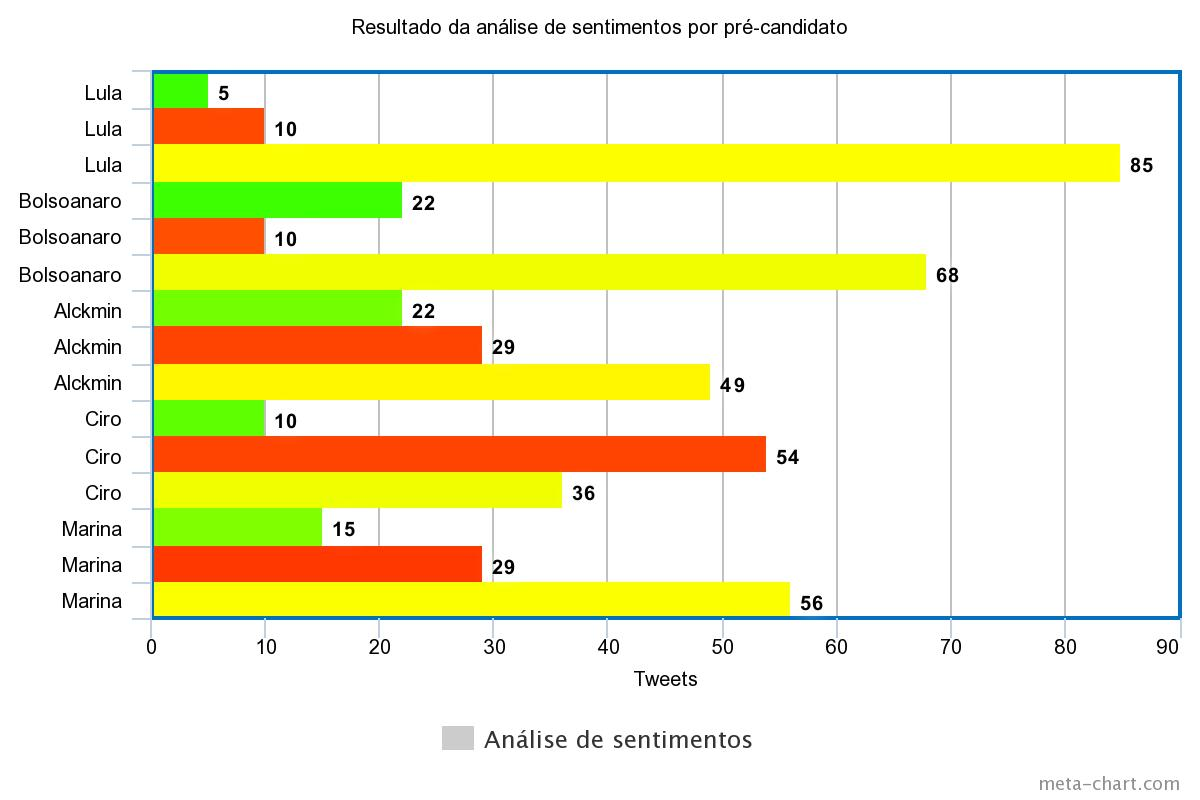
\includegraphics[width=0.95\textwidth]{imagens/resultadoSentimentoTwitter.jpeg}
        \caption {Quantidade de mensagens por sentimento do Twitter.}
        \source{Fonte: Criado pelo autor com auxílio da ferramenta meta-chart (2018)}
        \label{fig:resultadoSentimentoTwitter}
    \end{figure}

\subsection{Quantidade de dados por pré-candidato aleatória}

Foram coletados um total de 1977 \textit{tweets}, no dia  2 de Junho de 2018, das 21h às 22h (UTC), dos quais 303 forma relacionados aos cinco pré-candidatos deste estudo de caso. Pode-se observar que o pré-candidato Ciro Gomes, do PDT, possui o maior volume de dados relacionados a ele. Informação melhor observada na figura \ref{fig:resultSentimentoStreaming}.
    
    \begin{figure}[h]
        \centering
        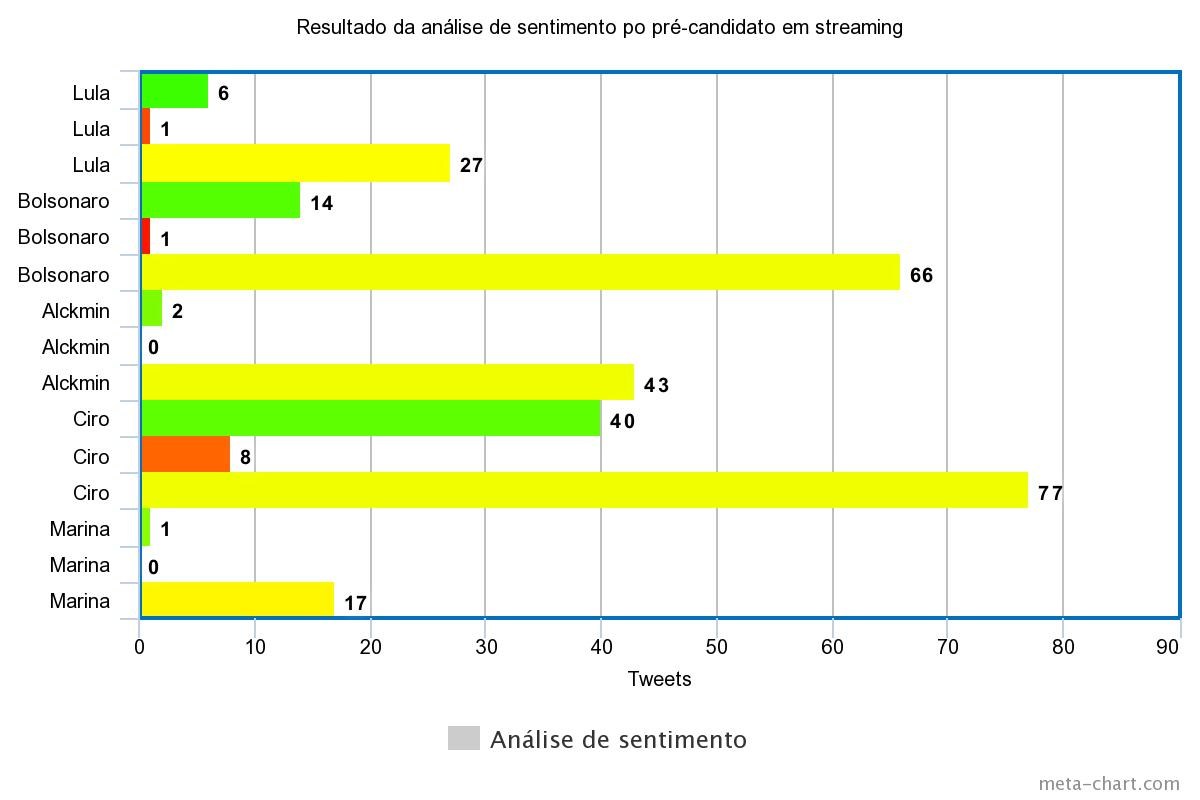
\includegraphics[width=0.95\textwidth]{imagens/resultSentimentoStreaming.jpeg}
        \caption {Quantidade de mensagens por sentimento do Twitter.}
        \source{Fonte: Criado pelo autor com auxílio da ferramenta meta-chart (2018)}
        \label{fig:resultSentimentoStreaming}
    \end{figure}

  \begin{table}[!htb]
       \textsf{\caption{Resultado da análise de sentimento em pré-candidatos, no Twitter, por \textit{streaming} de dados.}}
       \centering
       \medskip
    
        \begin{tabular}{ |p{4cm}|p{3cm}|p{3cm}|p{3cm}|  }
         \hline
         \multicolumn{4}{|c|}{Relação entre quantidade de sentimento pré-candidato} \\
         \hline
           \diagbox{Candidato}{Sentimento} & Postivo & Negativo & Neutro\\
         \hline
         
         \hline
          Lula (PT)   & 6 & 1 & 27  \\
         \hline
         
          \hline
          Bolsonaro (PSL)   & 14 & 1 & 66 \\
         \hline
         
          \hline
          Alckmin (PSDB)   & 2 & 0 & 43  \\
         \hline
         
          \hline
          Ciro (PDT)   & 40 & 8 & 77  \\
         \hline
         
          \hline
          Marina (REDE)   & 1 & 0 & 17  \\
         \hline
    
        \end{tabular}
        \label{table:streamingResultado}
    \end{table}

Dos quase 2 000 \textit{tweets} coletados, apenas 19 vieram com as coordenadas geográficas do usuário que postou, na rede social, no instante da postagem. Da resposta vinda da API do Twitter, o campo \textit{coordinates} contém essas informações. 

Apesar de ser pequeno, o volume de dados sobre localização, a figura \ref{fig:mapa}, mostra de que local do Brasil as mensagens foram postadas. Sendo os marcadores, que estão no mapa, de cor verde representando as mensagens positivas, de cor vermelha as negativas e azuis as mensagens neutras.

    \begin{figure}[h]
        \centering
        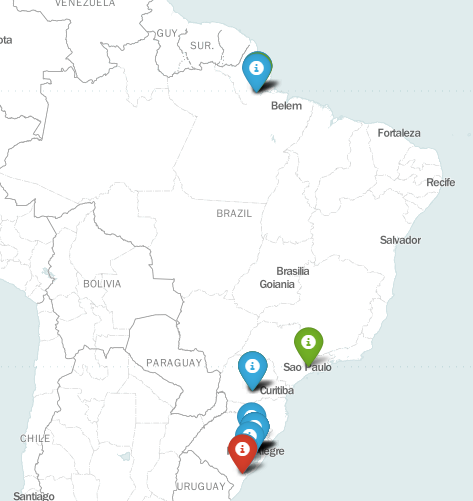
\includegraphics[width=9cm, height=9cm]{imagens/mapa.png}
        \caption {Locais do Brasil onde \textit{tweets} foram postados.}
        \source{Fonte: Criado pelo autor com auxílio da biblioteca folium (2018)}
        \label{fig:mapa}
    \end{figure}

    



        











